\chapter{Materials and Methods}

\section{Patients Characterization}

This study is part of the research project entitled "Clinical utility of liquid biopsy in non-small cell lung cancer patients with EML4-ALK translocation". Its objective is to determine the best strategy for the identification of EML4-ALK translocations and to assess the clinical utility of periodic tumor monitoring in ALK-positive NSCLC patients from liquid biopsies. In this context, between June 2015 and July 2019, several ALK-positive NSCLC advanced subjects were recruited from 6 hospitals across Spain, including the Hospital Universitario Puerta de Hierro, the Complejo Hospitalario Universitario A Coruña, the Hospital Universitario Fundación Jiménez Díaz, the Hospital Clínic Barcelona, the Hospital General Universitario de Alicante, and the Hospital General Universitario de Valencia.

The primary study was conducted under the precepts of the Helsinki Declaration and was approved by the Hospital Puerta de Hierro Ethics Committee (internal code 79-18). Patients were eligible if they consented to allow their clinical information to be used in the previously mentioned research project. Their clinical history was queried for information on the age of diagnosis, sex, smoking status, histology, stage, Eastern Cooperative Oncology Group (ECOG) performance status, and current therapies.

Eligible patients had histologically confirmed diagnosis of stage III–IV NSCLC that was ALK-positive, a measurable disease according to the response evaluation criteria in solid tumors (RECIST, version 1.1), were candidates to be treated with an ALK inhibitor, and were 18 years old or older. Exclusion criteria included the impossibility of frequent venipuncture or evidence of any other major clinical disorder or finding that would have made it undesirable for the patient to participate in the study.

Finally, for this project, a total of 39 liquid biopsies (37 plasma samples and 2 CSF samples) obtained from 30 patients who have met the above restrictions were used.

\section{Laboratory Procedures}

In order to identify the required parameters to design and implement the automatic algorithm for filtering genetic variants, several clinical procedures have been carried out, including the collection and conditioning of the ALK-positive NSCLC samples, their sequencing and analysis, and the subsequent confirmation of the identified mutations.

\subsection{Sample Collection and Processing}

Once an ALK gene mutation is diagnosed in a patient with NSCLC according to an anatomic pathology report (FISH and\slash or IHC), peripheral blood is drawn into a 9 $mL$ Streck Cell-Free DNA BCT\textsuperscript\textregistered{} (Streck, La Vista, NE, USA) tube and transported to the Liquid Biopsy Laboratory, where it is preserved until its processing. Within the context of the aforementioned project, blood samples have been extracted from patients in the pre-treatment stage, at months 2, 4, 6, 8, 12, 15 and 18, and at progression.

In this study, isolation of cfDNA and exosomes from the cellular fraction was achieved by two consecutive centrifugation processes at room temperature, the first at 1500 $g$ for 10 $min$ and the second at 5000 $g$ for 20 $min$. After discarding the supernatant containing the clean plasma, the last step of the cfDNA and exosome RNA isolation was performed using the QIAamp\textsuperscript\textregistered{} Circulating Nucleic Acid Kit (QIAgen, Valencia, CA, USA) and the exoRNeasy\textsuperscript\textregistered{} Serum/Plasma Maxi Kit (QIAgen, Valencia, CA, USA) respectively, following the manufacturer's instructions. Until library preparation for sequencing, processed samples were stored at $-80$ \textdegree{C}.

Regarding CSF samples, their processing was identical to that described for plasma. These were first collected in a 9 $mL$ Streck Cell-Free DNA BCT\textsuperscript\textregistered{} (Streck, La Vista, NE, USA) tube, and then the CSF nucleic acids were isolated using the QIAamp\textsuperscript\textregistered{} Circulating Nucleic Acid Kit (QIAgen, Valencia, CA, USA).

\subsection{Library Preparation}

NGS libraries were prepared from 10.4 $\mu L$ of cfDNA or exosome RNA using the Oncomine\texttrademark{} Pan-Cancer Cell-Free Assay (Thermo Fisher, Palo Alto, CA, USA) according to the manufacturer's instructions. This multi-biomarker amplicon-based assay is optimized to detect more than 900 hotspots in 52 key genes from liquid biopsy samples containing tumor-derived DNA and RNA. Additionally, it enables a limit of detection (LOD) down to 0.1\%, allowing the study of single-nucleotide variants (SNVs), short insertions and deletions (InDels), copy-number variations (CNVs), and fusions.

The steps that have been followed to prepare the NGS libraries are described below:

\begin{figure}[ht]
    \centering
    \begin{subfigure}{0.75\textwidth}
        \centering
        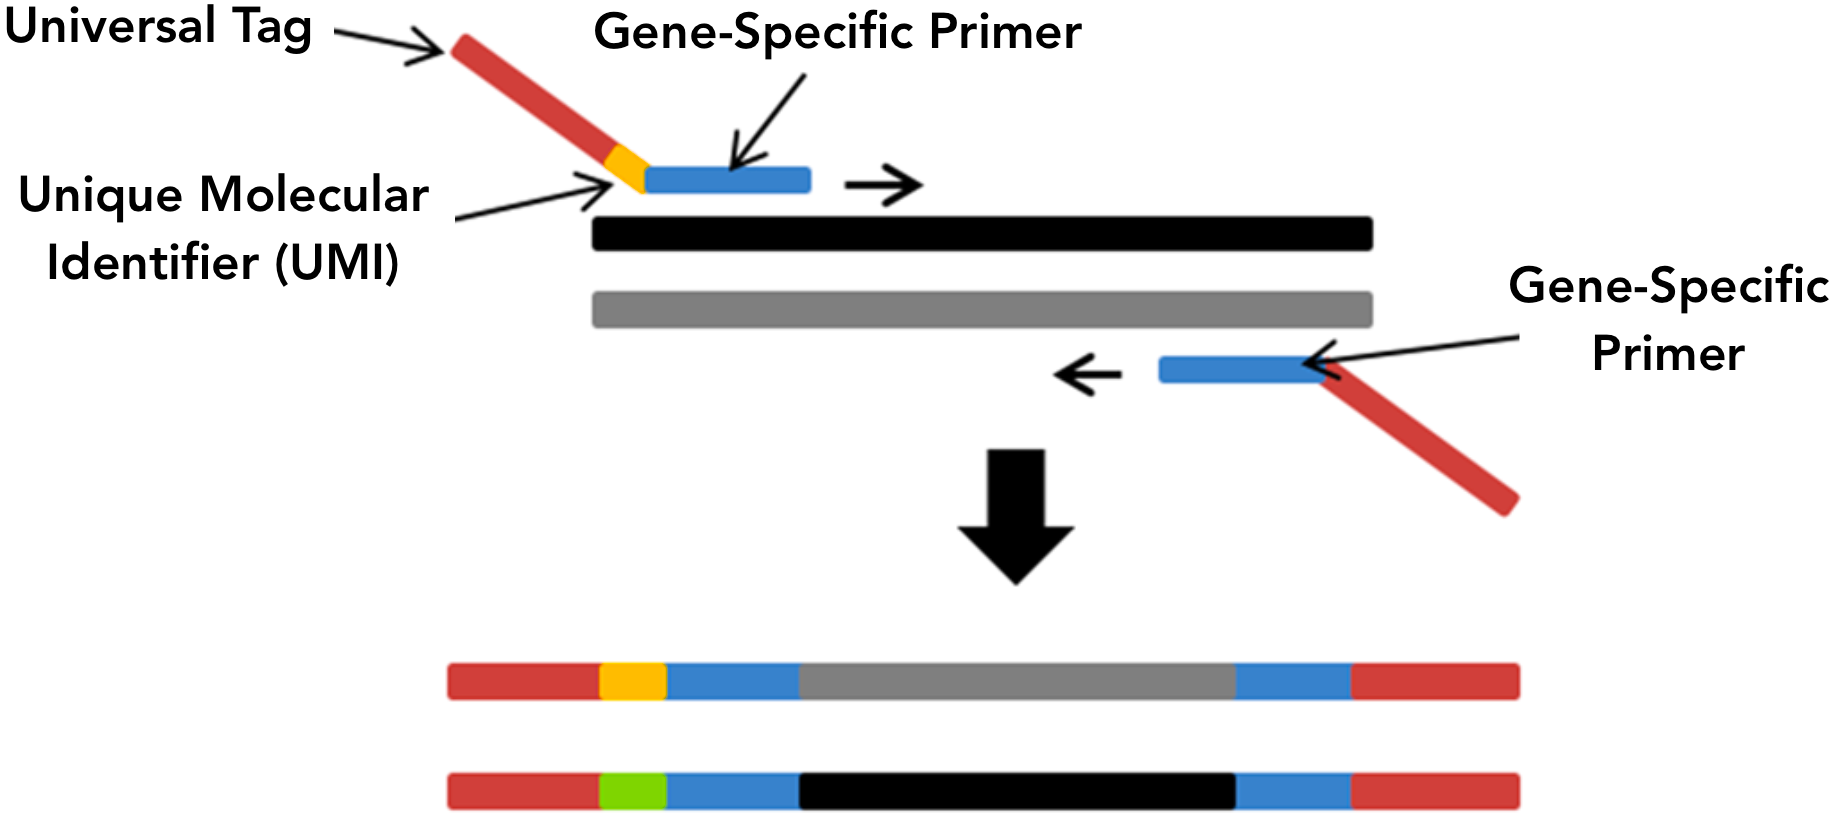
\includegraphics[width=\textwidth]{Images/chapter_3/library_prep_1.png}
        \caption{Incorporation of UMIs in two DNA fragments. This first PCR step assigns a random molecular barcode (UMI) to each of the DNA sequences, including gene-specific primers and a universal tag. \\}
        \label{fig:Library_1}
    \end{subfigure}
    \hfill
    \begin{subfigure}{0.95\textwidth}
        \centering
        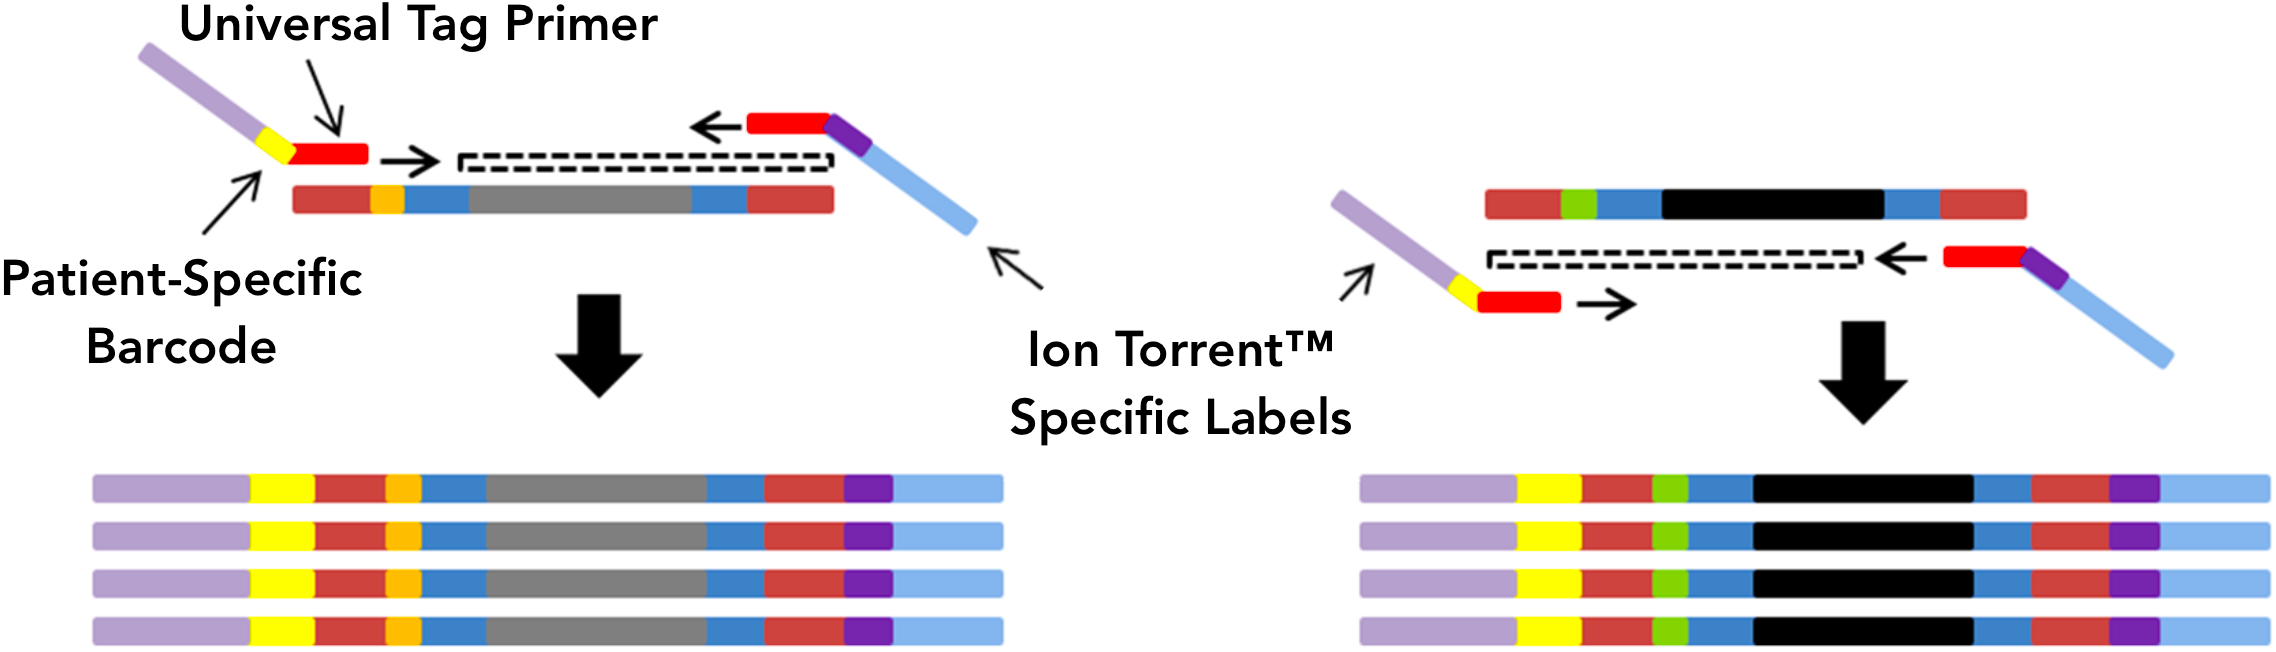
\includegraphics[width=\textwidth]{Images/chapter_3/library_prep_2.png}
        \caption{Amplification of the target amplicons. This second PCR uses custom primers to amplify the barcoded molecules with a universal tag sequence, adding patient-specific barcodes along with NGS-specific sequences.}
        \label{fig:Library_2}
    \end{subfigure}
    \hfill
    \caption{Schemes of the amplification and tagging technology used in in the Oncomine\texttrademark{} Pan-Cancer Cell-Free Assay. True hotspot variants can be distinguished from workflow errors by the frequency of variants in families that have the same UMI.}
    \label{fig:Library}
\end{figure}

\begin{enumerate}[font=\bfseries]
    \item \textbf{Reverse transcription of cell-free nucleic acids}. After isolating the free-circulating DNA and exosome RNA, complementary DNA (cDNA) was synthesized in this step. Specifically, the reverse transcription of exosome RNA was performed using the PrimeScript\texttrademark{} RT Reagent Kit (TaKaRa, Japan).
    \item \textbf{Target amplification}. After the fragmentation of the isolated and synthesized DNA using enzymatic methods, 2 cycles of tagging PCR were performed producing labeled DNA amplicons within a specific size range (\autoref{fig:Library_1}). In this sense, prior to target enrichment and library amplification, each original DNA molecule was assigned a random unique molecular identifier (UMI). This technology is aimed to detect, quantify, and sequence unique DNA fragments with high-resolution, allowing the identification and removal of amplification artifacts arising from library preparation. In addition, this ligated adapter also contains the first sample index and a universal tag.
    \item \textbf{Target amplicons purification}. Sample purification is a critical step for obtaining accurate NGS data. Therefore, a specific reagent with magnetic beads was used in this study to remove short primers, unincorporated deoxyribonucleotide triphosphates (dNTPs), enzymes, short-failed PCR products, and salts from the PCR reactions.
    \item \textbf{Amplification of the target amplicons with barcode adapted primers}. In this step, specific DNA adapter sequences were annealed to the 5' and 3' ends of the amplicon DNA, enabling the analysis of multiple samples simultaneously. Specifically, this second PCR (18 cycles) was performed to add patient-specific barcodes along with particular labels to create Ion Torrent\texttrademark{} sequencer-compatible libraries (\autoref{fig:Library_2}).
    \item \textbf{Barcoded library purification}. To guarantee reliable sequencing results, and in a process similar to the previous one, a purification of the barcoded amplicons was carried out.
    \item \textbf{Size selection}. To isolate the DNA fragment sizes of interest for efficient and high-quality DNA sequencing, magnetic beads with varying concentrations of buffers were used for size selection.
    \item \textbf{Library quantification}. To estimate the DNA concentration and to ensure equal representation of the indexed libraries, each of the samples was quantified with a qPCR system (40 cycles) and compared to the standard curve. Finally, the definitive barcoded libraries were pooled and adjusted to a final concentration of 50 $pM$.
\end{enumerate}

AMPure XP\textsuperscript\textregistered{} magnetic beads (Beckman Coulter, Inc., Brea, CA, USA) were used to carry out the purification and size selection steps, while the Ion Library TaqMan\texttrademark{} Quantitation Kit (Thermo Fisher, Palo Alto, CA, USA) and the StepOnePlus\texttrademark{} Real-Time PCR System (Thermo Fisher, Palo Alto, CA, USA) were used for the quantification.

\subsection{Template Preparation and Chip Loading}

Template preparation is based on an emulsion PCR (ePCR) method (\autoref{fig:ePCR}). It starts with the denaturation of the fragmented and ligated DNA, which is then mixed with beads. Each bead has thousands of copies of an oligonucleotide, which is complementary to one of the adapters and to which the corresponding DNA fragments will be attached by clonal amplification. Empty beads are discarded, remaining the rest of them in the chip wells (one bead per well).

\begin{figure}[ht]
    \centering
    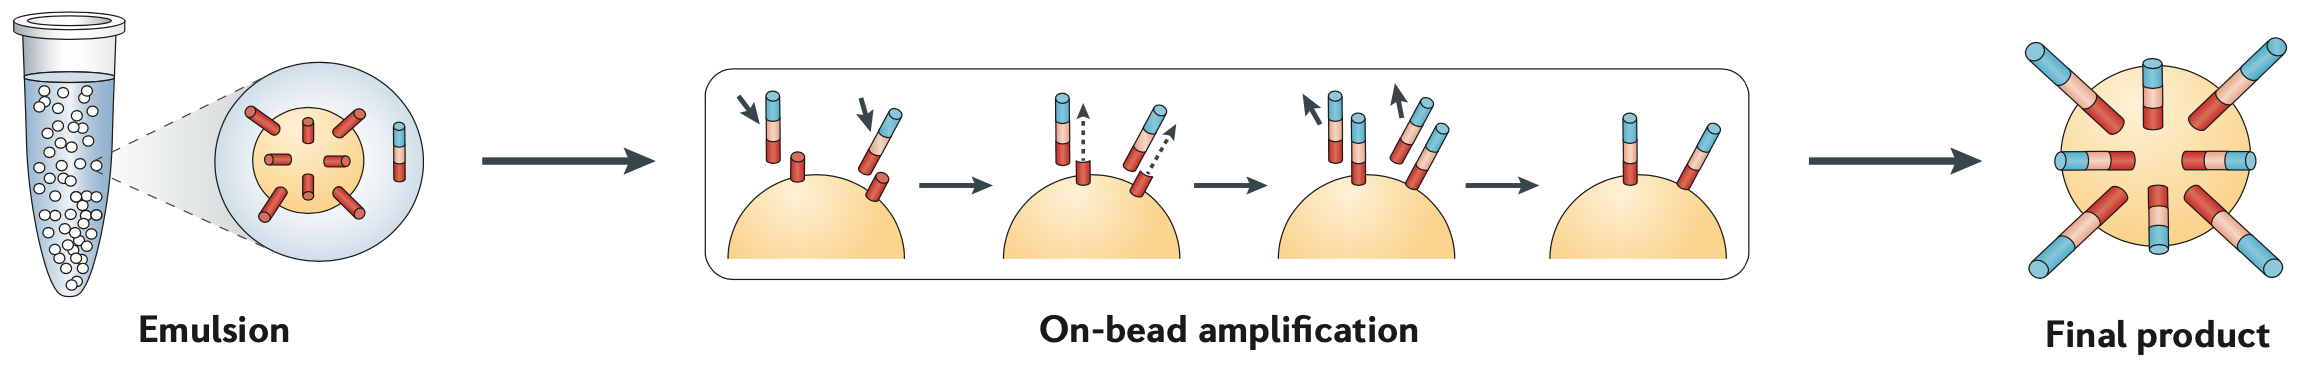
\includegraphics[width=\textwidth]{Images/chapter_3/ePCR.png}
    \caption{Ion Torrent\texttrademark{} template preparation technique. Micelle droplets are loaded with primers, complementary adapters, dNTPs, and DNA polymerase. Then PCR is carried out within the micelle, covering each bead (100–200 million of beads) with thousands of copies of the same DNA sequence. Modified image from \cite{NGS}.}
    \label{fig:ePCR}
\end{figure}

For both template preparation and chip loading, the Ion Chef\texttrademark{} System (Thermo Fisher, Palo Alto, CA, USA) was used. It automates these processes, loading up to 8 samples on a single Ion 550\texttrademark{} Chip (Thermo Fisher, Palo Alto, CA, USA), which is subsequently used for sequencing.

\subsection{Sequencing}

The previously loaded chips were sequenced on an Ion GeneStudio\texttrademark{} S5 Sequencer (Thermo Fisher, Palo Alto, CA, USA). It is a semiconductor-based NGS platform that decodes the template DNA sequence by detecting \ce{H^{+}} ions that are released upon the incorporation of nucleotides to the DNA fragment attached to its corresponding bead. 

\begin{figure}[ht]
    \centering
    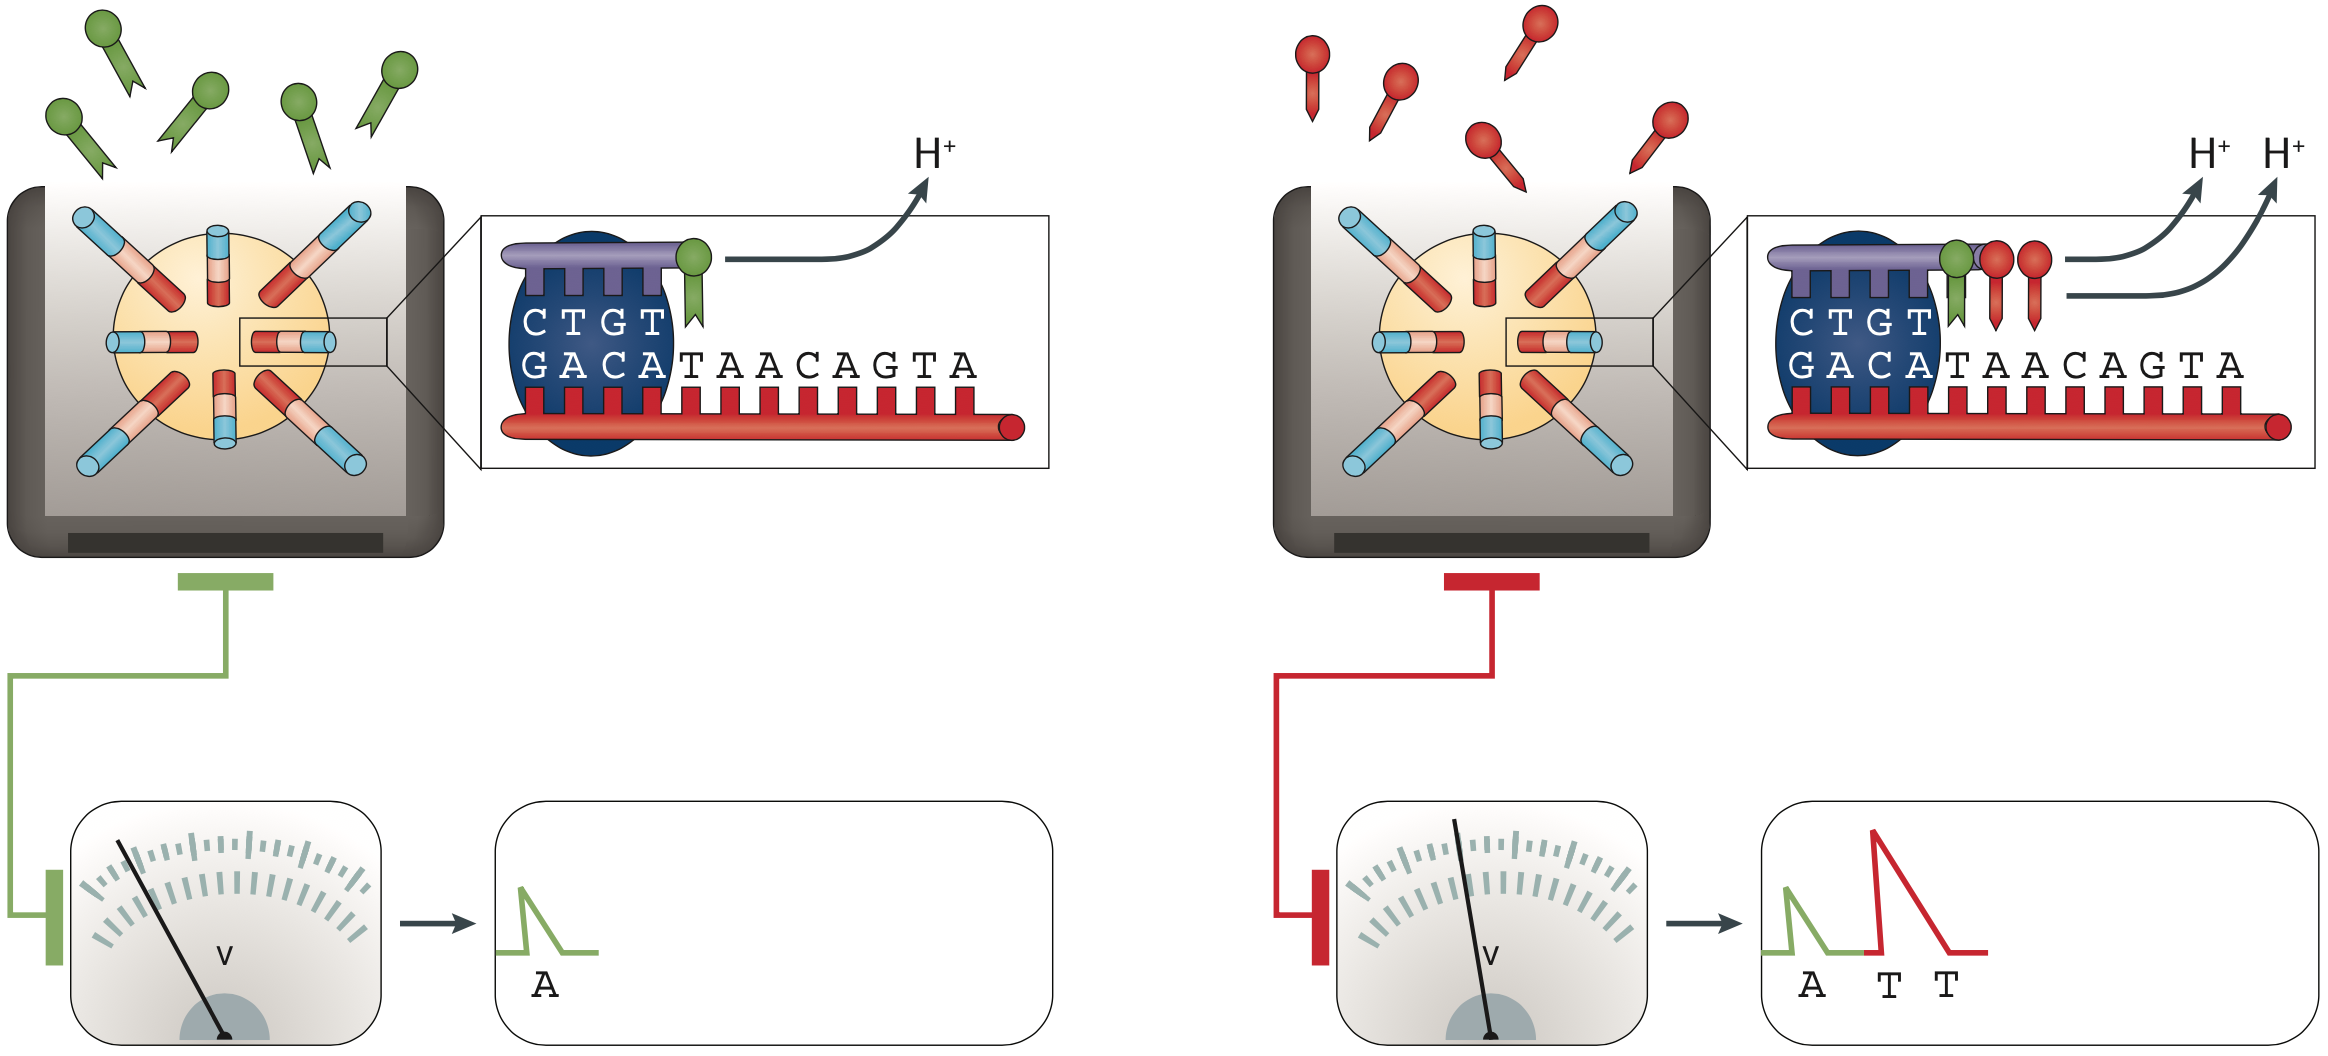
\includegraphics[width=\textwidth]{Images/chapter_3/NGS_sequencing.png}
    \caption{Ion Torrent\texttrademark{} measurement of nucleotide addition: incorporation of an adenine (A) followed by the addition of two thymines (T). Modified image from \cite{NGS}.}
    \label{fig:NGS_sequencing}
\end{figure}

This process occurs simultaneously in millions of wells, which contain template-attached beads incubated with DNA polymerase and a particular type of dNTP. Therefore, if that specific dNTP matches the growing template strand, the DNA polymerase adds it, resulting in a discharge of a \ce{H^{+}} ion that will change the pH of the solution in the well. This shift is recorded and converted to voltage, indicating that the nucleotide was incorporated and the base was called (\autoref{fig:NGS_sequencing}).

\subsection{Sequenced Data Analysis}

Data analysis was completed in two consecutive steps. First, a primary analysis was performed to study the overall quality of the sequenced data. Subsequently, the identified genetic variants were analyzed and verified using several software tools. In this last step, data of interest was also collected for the development of the algorithm.

\subsubsection{Primary Analysis}

The sequencing runs were scheduled with the Torrent Suite\texttrademark{} v5.12 software, generating at the end of the process a file with the main quality specifications (\autoref{fig:20200108_1}), which include:
\begin{itemize}
    \item \textbf{ISP loading density}. Percentage of chip wells that contain an Ion Sphere\texttrademark{} Particle.
    \item \textbf{Total reads}. The total number of reads associated with a specific barcode.
    \item \textbf{Read length ($\boldsymbol{bp}$)}. Length of the called reads.
\end{itemize}

\begin{figure}[ht]
    \centering
    \begin{subfigure}{0.85\textwidth}
        \centering
        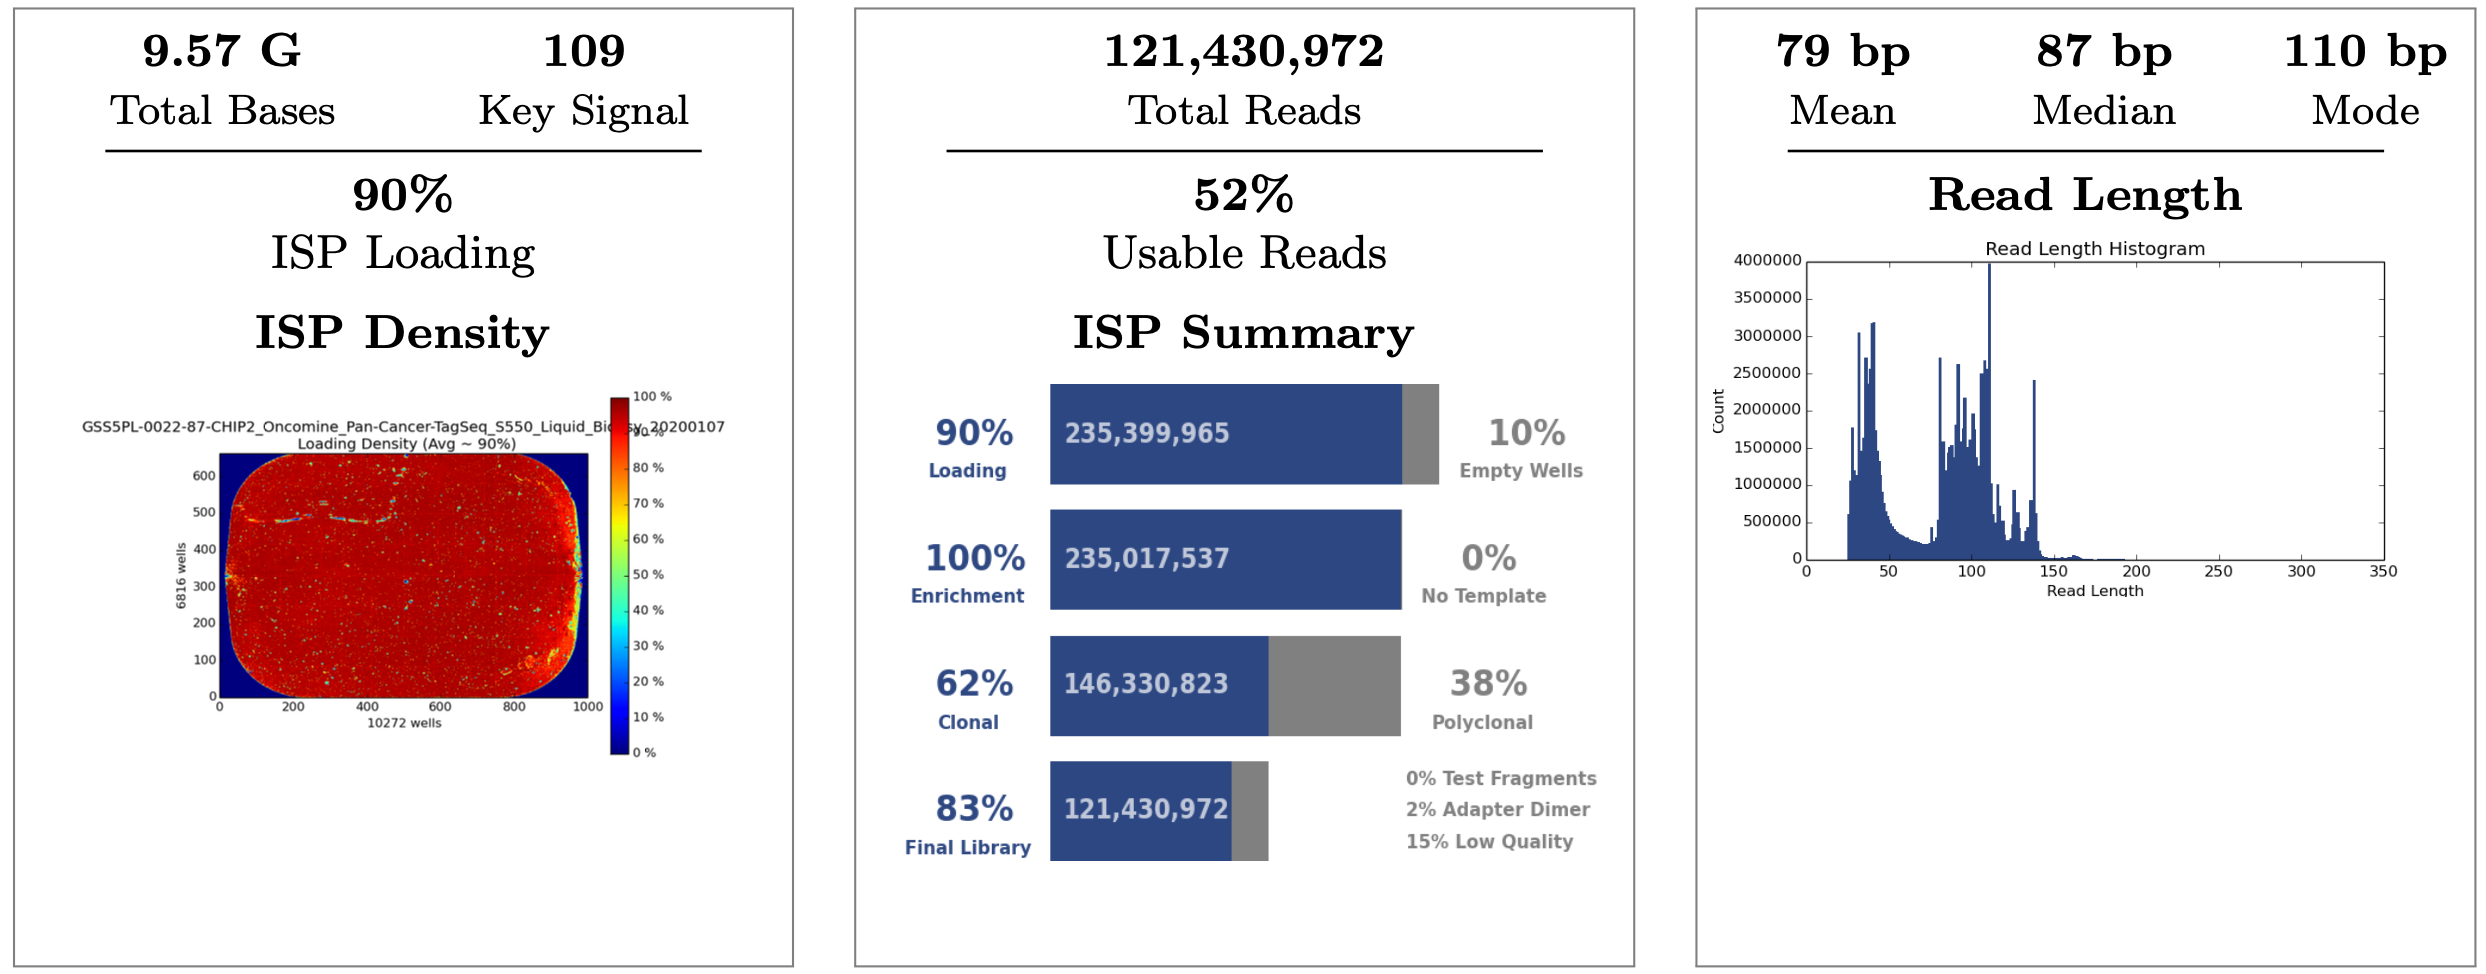
\includegraphics[width=\textwidth]{Images/chapter_3/20200108/20200108_1.png}
        \caption{Quality overview of a specific NGS run. The sequencing quality is directly proportional to the value of the ISP loading parameter. \\}
        \label{fig:20200108_1}
    \end{subfigure}
    \hfill
    \begin{subfigure}{0.85\textwidth}
        \centering
        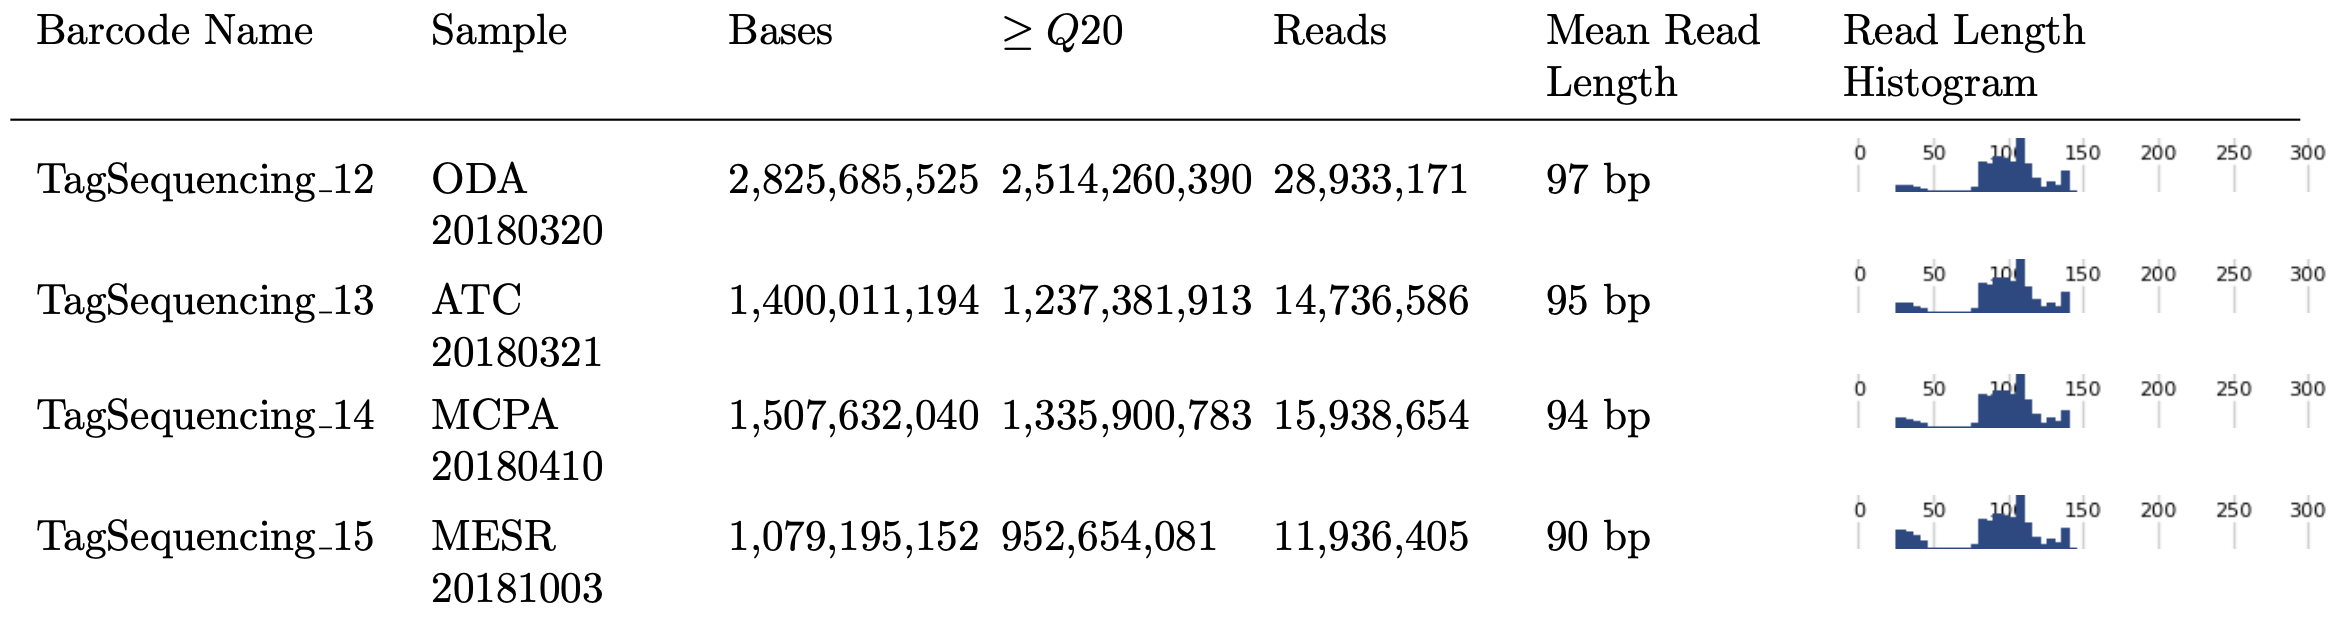
\includegraphics[width=\textwidth]{Images/chapter_3/20200108/20200108_2_v2.png}
        \caption{Quality parameters of 4 of the 8 sequenced samples. A Gaussian  base pair distribution in each of the histograms is indicative of well-prepared libraries.}
        \label{fig:20200108_2}
    \end{subfigure}
    \hfill
    \caption{Ion Torrent\texttrademark{} NGS run summary (NGS run ID: 20200108).}
    \label{fig:NGS_summary}
\end{figure}

Additionally, for each of the samples analyzed in the run (8 samples), the server generates an additional report with the following parameters (\autoref{fig:20200108_2}):
\begin{itemize}
    \item \textbf{Bases}. The number of base additions for each barcode.
    \item \textbf{$\boldsymbol{\ge}$ Q20}. The number of reads that have a predicted quality score of Q20 or better.
    \item \textbf{Reads}. The total number of filtered and trimmed library reads.
    \item \textbf{Mean read length ($\boldsymbol{bp}$)}. Average read length.
\end{itemize}

This raw data was processed automatically on the Torrent Server\texttrademark{} v5.12 and then aligned to the reference hg19 genome. In this context, to study the sequence coverage for target genomic regions, the Coverage Analysis Plugin v5.12.0.0 was used, obtaining the following parameters (\autoref{fig:20200108_4}):
\begin{itemize}
    \item \textbf{Mapped reads}. The total number of reads that were mapped to the reference.
    \item \textbf{On target (\%)}. Percentage of reads that were mapped to any targeted region.
    \item \textbf{Mean depth}. The average number of reads that align to known reference bases.
    \item \textbf{Uniformity (\%)}. Percentage of bases, in all targeted regions, that is covered by at least 20\% of the average base coverage depth reads.
\end{itemize}

\begin{figure}[t]
    \centering
    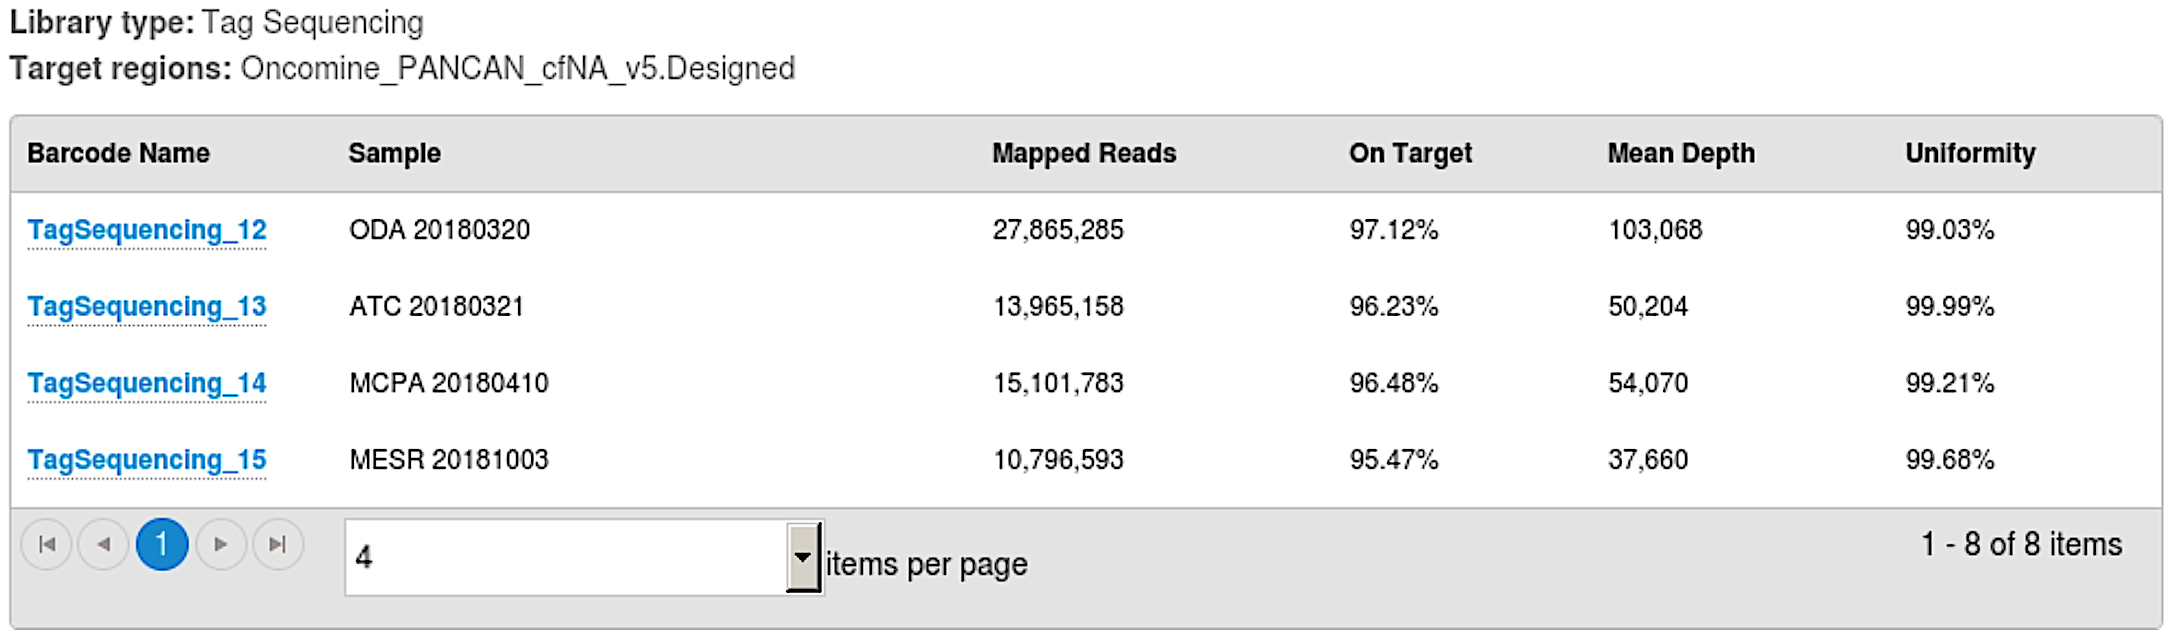
\includegraphics[width=\textwidth]{Images/chapter_3/20200108/20200108_4_v2.png}
    \caption{Coverage Analysis Plugin output parameters of 4 of the 8 sequenced samples (NGS run ID: 20200108). Successful sequencing shows a percentage of reads mapped to target regions and uniformity values close to 100\%.}
    \label{fig:20200108_4}
\end{figure}

\subsubsection{Secondary Analysis} \label{Secondary_analysis}

After ensuring that the sequencing had been performed as expected, the resulting data of the quality control passing samples were uploaded in BAM format to the Ion Reporter\texttrademark{} v5.12. Variant calling, annotation, and filtering were performed on this platform using the Oncomine\texttrademark{} TagSeq Pan-Cancer Liquid Biopsy v2.1 workflow, including this pipeline analysis the mapping of the sequenced reads to defined target regions (Oncomine\texttrademark{} Pan-Cancer DNA Regions v$1.0$) and the variant calling using the Oncomine\texttrademark{} Variant Annotator v2.3 plugin. For each of the samples the following parameters were obtained:
\begin{itemize}
    \item \textbf{Median read coverage}. Median coverage across targets.
    \item \textbf{Median molecular coverage}. The median number of individual interrogated DNA molecules across targets.
    \item \textbf{Limit of Detection (LOD)}. Numeric range (\%) where the minimum represents the median value across all targets and the maximum represents the LOD for the $80^{th}$ percentile targets.
\end{itemize}

For sensitive variant detection down to 0.1\% frequency, optimal results are obtained when targeting a median read coverage $> 25000$, median molecular coverage $> 2500$, and both numbers of the LOD segment are $\le 0.1\%$ \cite{Oncomine_PanCancer}.

Furthermore, with the Ion Reporter\texttrademark{} platform, it was possible to identify and analyze each of the deviations from a reference genome based on their biological and clinical relevance, obtaining information about the gene, the location, the allele frequency, and the specific type of each variant. The main parameters of interest for each of these mutations were:
\begin{itemize}
    \item \textbf{Molecular depth}. The number of interrogated DNA molecules containing target.
    \item \textbf{Molecular counts}. The number of detected DNA molecules containing a variant allele.
\end{itemize}

On the other hand, it is possible to download all this raw data in a \textit{.tsv} file, which includes an even more detailed analysis of all the variants. This file is precisely the one that was used to design the bioinformatic pipeline, along with the parameters described above.

Finally, all candidate mutations were manually reviewed using the Integrative Genomics Viewer (IGV) v2.3.40 to be subsequently confirmed by dPCR.

\subsection{Confirmation of the Sequenced Results}

Digital PCR is a tool that is used to improve the efficiency of the NGS workflow and for the verification of sequencing data. In this study, the previously identified mutations (\autoref{Secondary_analysis}) in the cfDNA or cDNA samples were confirmed by the QuantStudio\textsuperscript\textregistered{} 3D Digital PCR System (Applied Biosystems, South San Francisco, CA, USA) according to the manufacturer's specifications. The reverse transcription of exosome RNA to synthesize cDNA was performed using the PrimeScript\texttrademark{} RT Reagent Kit (TaKaRa, Japan).

Briefly, dPCR is based on the fact that the random distribution of molecules in many partitions follows a Poisson distribution. Each partition, which contains a specific labeled DNA sequence, acts as an individual and isolated PCR reaction. After amplification, the augmented target sequences are detected by fluorescence, which is sufficient to determine their concentration. In this study, this process was carried out following the next steps:
\begin{enumerate}[font=\bfseries]
    \item \textbf{Set up of the dPCR reaction}. It was performed by mixing a specific sample with the master mix and the assays, obtaining a final volume of 18 $\mu L$. Specifically, this reaction included 8.55 $\mu L$ of template cfDNA or cDNA, 9 $\mu L$ of 20X QuantStudio\texttrademark{} 3D Master Mix and 0.45 $\mu L$ of 40X TaqMan\texttrademark{} assays (predesigned TaqMan\texttrademark{} Liquid Biopsy dPCR assay and custom TaqMan\texttrademark{} assay). These assays include specific primers and labeled probes that have a fluorescent reporter dye (VIC\texttrademark{} or FAM\texttrademark{}) attached to its 5' end, and a quencher dye at its 3' end (ROX\texttrademark{}). In all assays, probes complementary to mutated and wild type (WT) DNA sequences were labeled with the FAM\texttrademark{} and VIC\texttrademark{} dye respectively.
    \item \textbf{Chip loading}. 14.5 $\mu L$ of the dPCR reaction was loaded using the QuantStudio\texttrademark{} 3D Digital PCR Chip Loader into the QuantStudio\texttrademark{} 3D Digital PCR 20K Chip v2, which has 20000 wells containing a DNA molecule that will be amplified independently in the thermocycling phase. In addition, positive and negative controls were included in each dPCR run to ensure that the primers have attached to the DNA strand and that there has been no foreign DNA contamination.
    \begin{figure}[t]
        \centering
        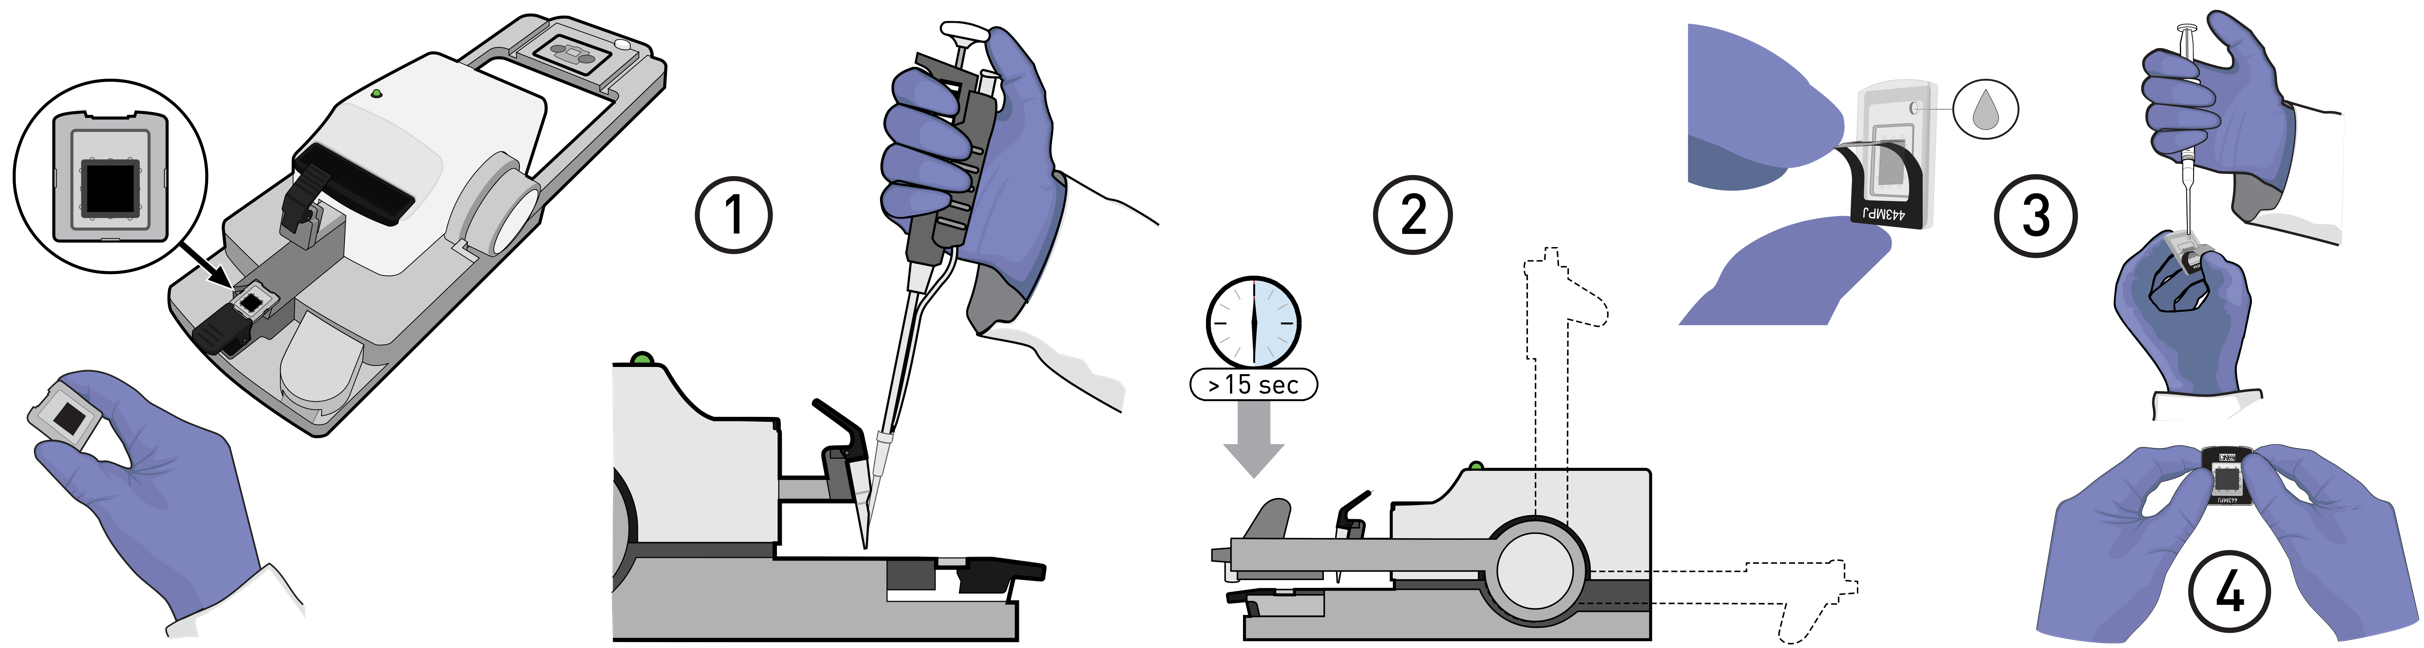
\includegraphics[width=\textwidth]{Images/chapter_3/chip_loading.png}
        \caption{ Chip loading. Charging of the dPCR reaction into the QuantStudio\texttrademark{} 3D Digital PCR 20K Chip v2 (1), lid application (2), filling of the assembly with Immersion Fluid (3), and sealing of the loading port (4). Modified image from \cite{dPCR_QuantStudio}.}
        \label{fig:Chip_loading}
    \end{figure}
    \item \textbf{Thermocycling}. This process, which was divided into 3 consecutive stages, was carried out with the QuantStudio\textsuperscript\textregistered{} 3D Digital PCR System (Applied Biosystems, South San Francisco, CA, USA). The temperature, duration, and number of cycles for each of the stages are summarized in \autoref{tab:dPCR_stages}. During the amplification stage, the Taq polymerase enzyme cleaves the aforementioned FAM\texttrademark{} and VIC\texttrademark{} bound probes, generating fluorescent signals that will be recorded and associated with specific wells on the chip in the next step.
    \begin{table}[ht]
        \centering
        \renewcommand{\arraystretch}{1.3}
        \begin{tabular}{ccccc}
        \rowcolor[HTML]{C0C0C0} 
        \textbf{Stage 1} & \multicolumn{2}{c}{\cellcolor[HTML]{C0C0C0}\textbf{Stage 2}} & \multicolumn{2}{c}{\cellcolor[HTML]{C0C0C0}\textbf{Stage 3}} \\
        \rowcolor[HTML]{FFFFFF} 96 \textdegree{C} & 56 \textdegree{C} & 98  \textdegree{C} & 72 \textdegree{C} & 22 \textdegree{C} \\
        \rowcolor[HTML]{EFEFEF} 10 $min$ & 2 $min$ & 30 $s$ & 10 $min$ & 30 $min$ \\
        \rowcolor[HTML]{FFFFFF} 1 cycle (hold) & \multicolumn{2}{c}{\cellcolor[HTML]{FFFFFF}40 cycles} & \multicolumn{2}{c}{\cellcolor[HTML]{FFFFFF}1 cycle (hold)}
        \end{tabular}
        \caption{Digital PCR reaction conditions used in this study for DNA denaturation, annealing, and elongation stages.}
        \label{tab:dPCR_stages}
    \end{table}
    \item \textbf{Chip reading}. After completing the thermocycling process, the chips were loaded into the QuantStudio\texttrademark{} 3D Digital PCR Instrument to read their fluorescence. This reading was performed twice to ensure that the subsequent data review is accurate and reliable.
    \item \textbf{Results interpretation}. The previously processed data was visualized and analyzed using the QuantStudio\texttrademark{} 3D Analysis Suite\texttrademark{} Cloud Software (\autoref{fig:FAM_VIC}). In this context, samples with a mutant allele fraction (MAF) equal to or higher than 0.1\% were considered positive (\autoref{eq:MAF}). Additionally, the LOD was assessed for all individual assays, being lower than 0.1\% in all cases.
    \begin{align} \label{eq:MAF}
        MAF &= \frac{FAM_{copies}/\mu L}{FAM_{copies}/\mu L \ + \ VIC_{copies}/\mu L} \\
        \text{where}~
        FAM_{copies} &\equiv \text{Number of reads of the mutated sequences} \notag \\
        VIC_{copies} &\equiv \text{Number of reads of the WT sequences} \notag
    \end{align}

    \begin{figure}[t]
        \centering
        \begin{subfigure}{0.30\textwidth}
            \centering
            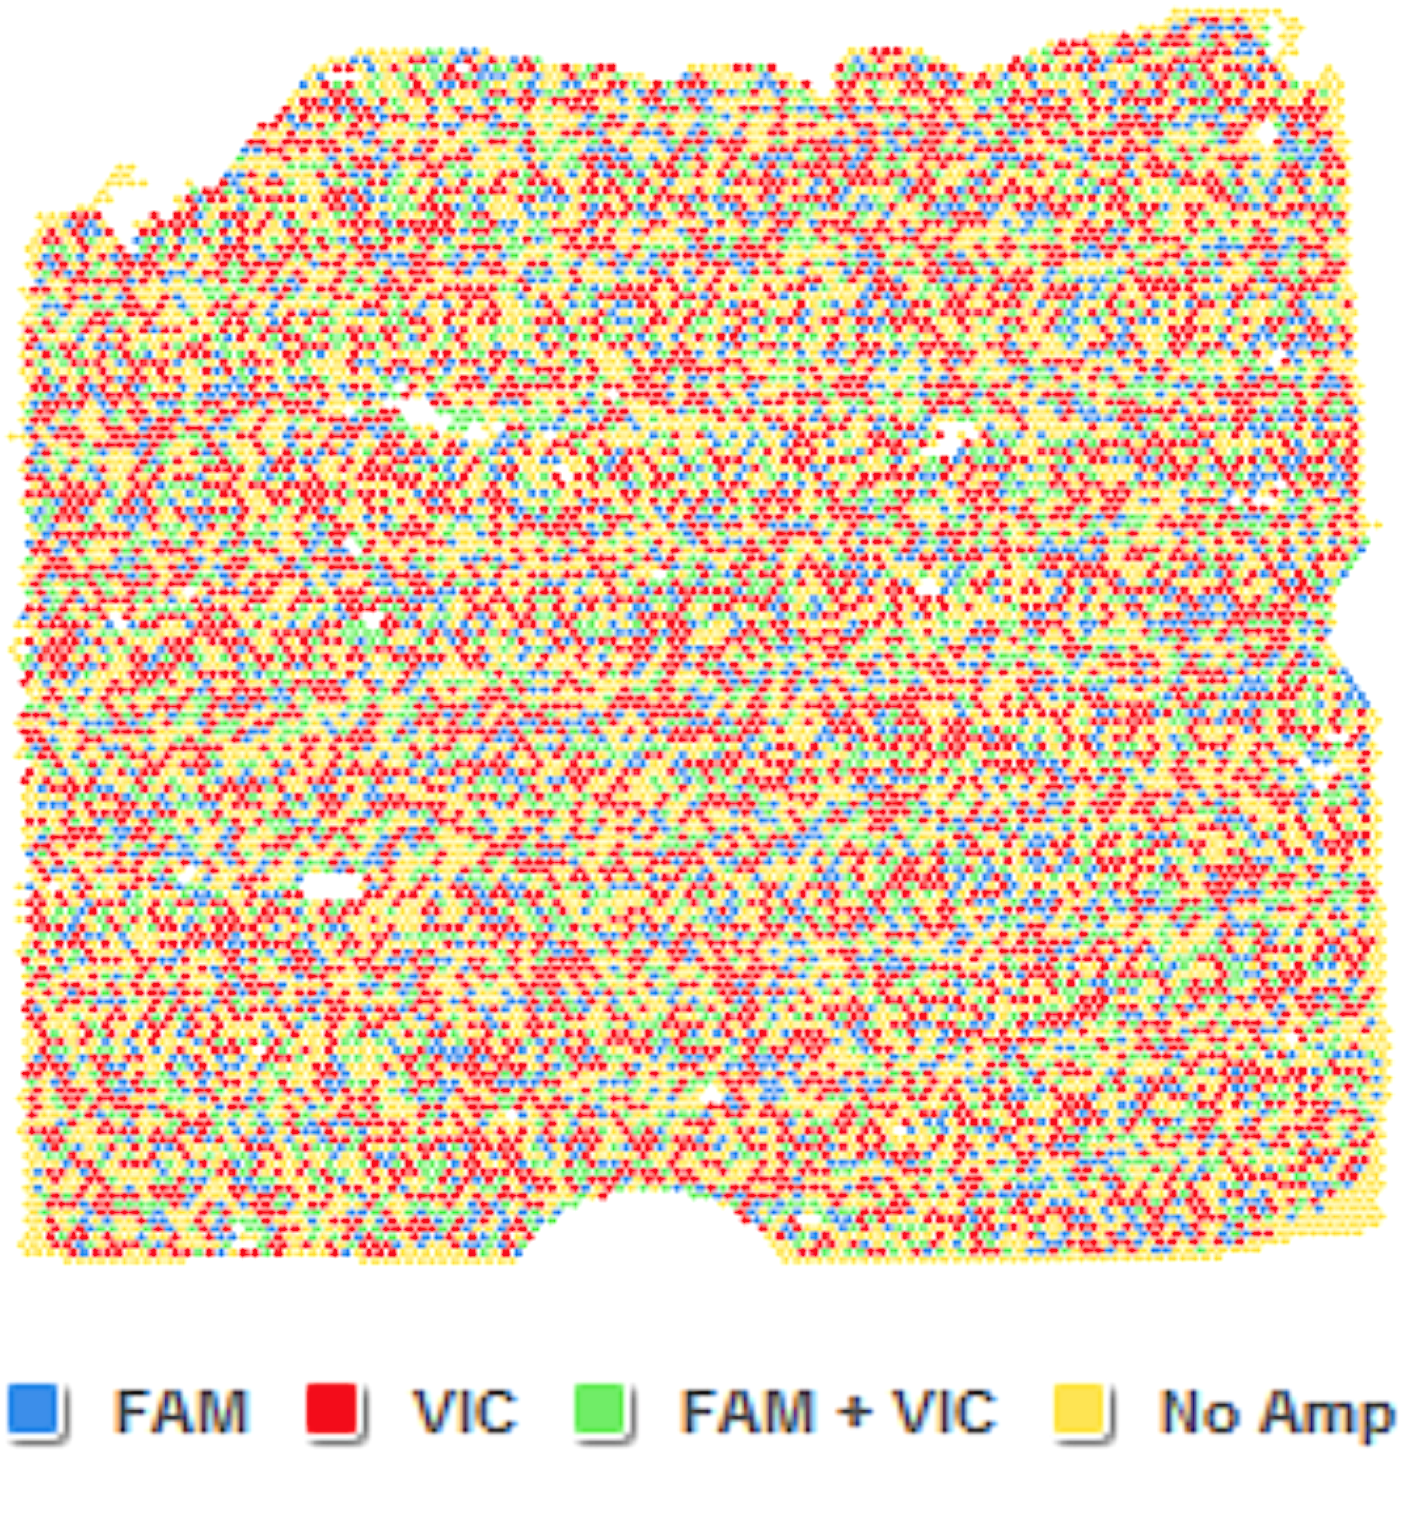
\includegraphics[width=\textwidth]{Images/chapter_3/FAM_VIC_chip.png}
            \caption{Chip view.}
            \label{fig:FAM_VIC_chip}
        \end{subfigure}
        \hfill
        \begin{subfigure}{0.69\textwidth}
            \centering
            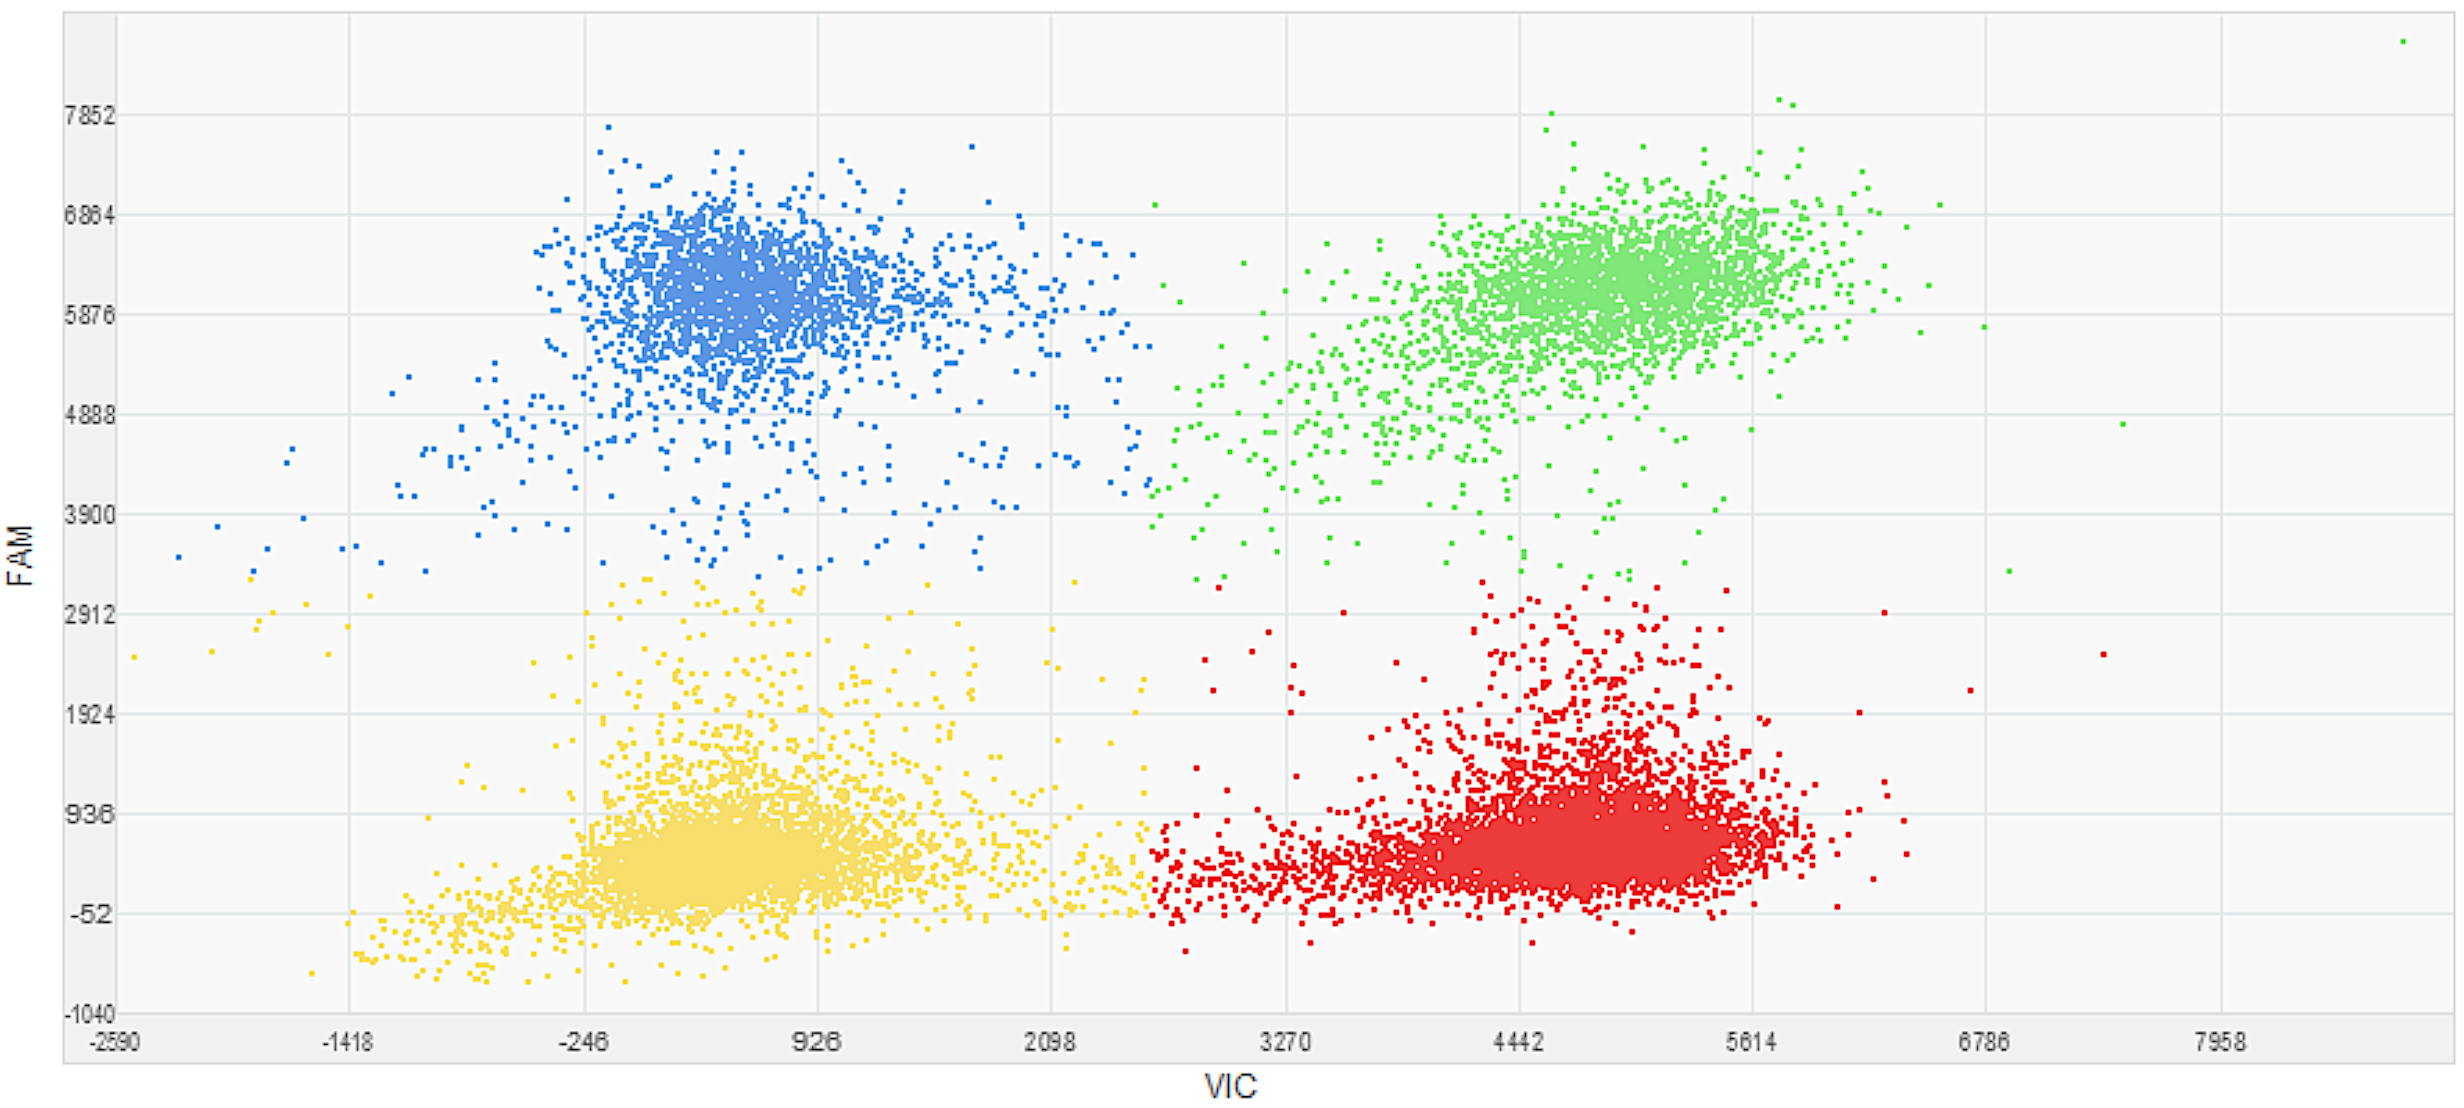
\includegraphics[width=\textwidth]{Images/chapter_3/FAM_VIC.png}
            \caption{FAM\texttrademark{} (Y-axis) vs. VIC\texttrademark{} (X-axis) view. A mutation has been detected if the blue cluster is identifiable in the dispersion chart.}
            \label{fig:FAM_VIC_dispersion}
        \end{subfigure}
        \hfill
        \caption{Quality and calls review of the dPCR. The red, blue, and green colors correspond to the VIC\texttrademark{} (fluorescence of the WT sequences), FAM\texttrademark{} (fluorescence of the mutated sequences), and VIC\texttrademark{}+FAM\texttrademark{} groups respectively, while the yellow represents the wells without amplification.}
        \label{fig:FAM_VIC}
    \end{figure}
\end{enumerate}

\section{Algorithm Specifications and Requirements}

The main objective of the developed algorithm is to fully automate the mutation filtering that is carried out before its ultimate confirmation by dPCR. In this way, this solution aims to simplify and automate the analysis of the NGS data described in \autoref{Secondary_analysis}. Eventually, this will save time, remove the human factor, and therefore improve the quality and efficiency of the entire process.

The different parameters of the proposed algorithm were identified according to the confirmed variants, both positive and negative, obtained from the liquid biopsy samples used in this study. To find specific patterns, each type of these clinically relevant deviations from a reference genome were studied individually using the obtained specifications described in \autoref{Secondary_analysis} and the \textit{non-filtered-oncomine.tsv} output file, which is generated after each sequencing. It contains both variants that have passed the Ion Reporter\texttrademark{} internal filter (Oncomine\texttrademark{} Variants v5.12) and initially discarded mutations. Therefore, apart from discerning whether a reading of an allele fraction represents a true mutation or is an artifact that should be ignored, the developed algorithm in this study will also be able to identify samples that have been initially discarded by the filters of the Ion Reporter\texttrademark{} platform, but are liable to be false-negatives.

This analysis and identification of the filtering parameters has been carried out with respect to each type of variant found during the study, including:
\begin{itemize}
    \item Fusions.
    \item Copy-number variations (CNVs).
    \item Single-nucleotide polymorphisms (SNPs).
    \item Insertions and deletions (InDels).
    \item Multiple-nucleotide polymorphisms (MNPs).
\end{itemize}

For each of them, minimum standards have been established to consider them valid and proceed with their confirmation by dPCR. Specifically, parameters such as the overall error of the NGS assay, the limit of detection (LOD), the coverage depth, the percentage of targeted bases sequenced at that coverage depth, the total number of target reads covering a variant region, the number of reads supporting a specific variant, and the clinical significance, among others, have been taken into account for the selection of the different thresholds.

Regarding the technical requirements, the programming language used in this study was \textsf{R} (v3.6.3), a free software environment for statistical computing and graphics. Furthermore, its capabilities were extended through additional packages:
\begin{itemize}
    \item \textbf{Tcl\slash Tk package}. Tcl is a general-purpose multi-paradigm system scripting language that provides the ability for applications to communicate with each other, while Tk is a cross-platform widget toolkit used for building graphical user interfaces (GUIs). It is included with the installation of \textsf{R}.
    
    In this thesis, the Tcl\slash Tk package was used to offer the end-user an intuitive graphical interface to carry out the entire filtering process, including loading the \textit{non-filtered-oncomine.tsv} files, selecting the type of variants to filter by, and saving mutations susceptible to being positive.
    \item \textbf{Scales (v1.1.1) package}. It contains functions that convert data values to perceptual properties. 
    
    In this particular case, it was used to transform the raw data obtained from the \textit{non-filtered-oncomine.tsv} files into interpretable values for the end-user.
\end{itemize}

Finally, to make programming more user-friendly through a graphical interface for \textsf{R}, the integrated development environment RStudio\textsuperscript\textregistered{} Desktop v1.2.5033 was used.